In \cref{sec:pert_flow} the perturbative behavior of the expectation value of the dimensionless quantity  $t_f^2\langle E \rangle$ was introduced. In this chapter the same object is studied using the data generated from our ensembles of lattice gauge field configurations, that our program generated. The matching between the perturbative and lattice results is also discussed.

\section{Discretization Effects on $t_f^2\langle E \rangle$}
\label{sec:scale}
The dimensionless observable $t_f^2\langle E \rangle$, as a first approximation, is proportional to the running coupling of the theory, see \cref{sec:pert_flow}. By plotting its value  as a function of the dimensionless quantity $t_f/r_0^2$ many interesting properties can be observed. First let us remember that $r_0=0.5$ fm is the Sommer parameter, described in \cref{sec:scale_fixing}, that has units of length.

\fig[0.7]{results/t2E.pdf}{$t_f^2\langle E \rangle$ computed on the four ensembles that were generated (\cref{MC:params}) as a function of the flow time in units of $r_0^2$. The solid line is for $t_f^2\langle E \rangle = 0.3$}{fig:t2E}

Firstly, the data suggests that for $t_f > 0.05r_0^2$ is the quantity $t_f^2\langle E \rangle$ is lattice spacing independent, and so is the coupling independent since they are related. This implies, as it was suggested by \cite{luscher_properties_2010}, that this quantity can be used to set the reference scale of the lattice, similarly to $r_0$. By selecting a value for $t_f^2\langle E \rangle$ one can create a reference scale. It was proposed to use the value of $0.3$, which from the plot we can see that is in the region of best matching between the different data series. The value must not be to small, as large discretization effects would affect the correct estimation of the quantity on the lattice.\\
In an operative way one finds the value of the flow time $t_0$ for which:
\beq
    t_0^2\langle E \rangle = 0.3
\eeq
This value, in this work, is found by selecting the 20 points, for each data series corresponding to a different $\beta$ value, and fitting a straight line through them. By inverse regression the value of $t_0$ and its uncertainty are found.\\
To check the validity of the assumptions, we can plot the analog of \cref{luscher:tsquareE} in which the ratio of $\sqrt{8t_0}/r_0$. This should have a well defined continuum limit, 
\fig[0.7]{results/EnergyContLimit.pdf}{Continuum limit extrapolation of the ratio $\sqrt{8t_0}/r_0$. The solid line is the linear fit of the data points, each representing a different $\beta$ value. The errorband is the $1\sigma$ confidence interval and the black point is the extrapolated continuum point. The fit is performed using $(a/r_0)^2$ to scale to the continuum.}{fig:energy_cont}
With this procedure we fix a value of $\sqrt{8t_0}/r_0$ to be:
\beq
\sqrt{8t_0}/r_0 = 0.951(5)
\eeq 
which is very close to the value found in \cite{ce_non-gaussianities_2015} of $\sqrt{8t_0}/r_0 = 0.941(7)$. It should be noted however that different procedures to extrapolate the continuum limit have been applied in this work and in the reference. We are for example neglecting the systematic uncertainty on $r_0$, while in \cite{ce_non-gaussianities_2015} all uncertainties are handled.
 
\section{Matching Perturbative and Lattice Results}
When focusing on the low flow time section of the $t_f^2\langle E \rangle$ plot, one can study the matching between the perturbative expansion of the observable, performed in \cref{energy_flow}, and the lattice results that we generated. \\
The greatest challenge however is that the flow time interval in which this matching happens is unknown. Certainly for large $t_f$ perturbation theory fails to describe the system: any perturbative expansion in $\alpha_s(q)$ becomes meaningless, as $q=1/\sqrt{8t_f}$ becomes small the coupling grows and approaches one. For small flow times in principle perfect agreement should be found up to an arbitrary scale. In practice the lattice results become unreliable in the sense that recovering the continuum limit correctly becomes hard. A a better understanding can be obtained by looking at a zoomed version of \cref{fig:t2E}. Both of these two bounds, no matter how intuitive they appear, are also not clearly defined and so no unique procedure can be found to constrain the matching region.
\fig[0.7]{results/t2EZoom.pdf}{Detail of \cref{fig:t2E} for small flow times.}{fig:t2EZoom} 

\subsection{Strategy for the Estimation of the Scale Energy $\Lambda$}
The problem we are interested to solve is to extract the value of the scale energy of Yang-Mills theory from the lattice data. The only link between the two is \cref{energy_flow}. If the equation is rewritten as:
\beq
t_f^2\langle E \rangle = \frac{3}{4\pi } \alpha_s(q) \left[ 1 + k_1\alpha_s(q) + \mathcal{O}(\alpha_s^2) \right],~~~~~k_1 = 1.0978% + 0.0075\times N_f
\label{eq:t2Ebuona}
\eeq  
one can compute the left hand side on the lattice and fit it to the analytic expression on the right hand side from perturbation theory. \\
As mentioned earlier the problem is to determine matching region, which now affects the fit range. This must be done carefully in order to prevent possible biases and to assess the error on $\Lambda$ properly. The first thing to do is to reconstruct the continuum limit curve for $t_f^2\langle E \rangle$. This has been done by selecting linearly spaced values of $t_f/r_0^2$ from $0.005$ to $0.085$ with spacing of $5\cdot 10^{-4}$. For each of the $\beta$ values, the ten closest points around every value of the linear space were used to fit a straight line and interpolate the value of  $t_f^2\langle E \rangle$ exactly on the point. An example for one of those points is shown in \cref{fig:interpolation}
 
\fig[0.7]{results/Interpolation.pdf}{Interpolation of the lattice data for $t_f^2\langle E \rangle$ around the point $t_f/r_0^2=0.04$. The solid color lines represent the linear fits on the data for one $\beta$ value each. The data points are the ten closest points to the desired value, represented by the black solid line.}{fig:interpolation}

With the interpolated data the continuum limit is taken for each value of the linear space by extrapolating the interpolated points to zero, \cref{fig:extrapolation}
\fig[0.7]{results/Extrapolation.pdf}{Extrapolation of the continuum limit for $t_f^2\langle E \rangle$ around the point $t_f/r_0^2=0.04$. The data points are the result of the interpolation procedure in \cref{fig:interpolation}. The line in red is the fit including all the ensembles that we considered, the line in blue excludes the $\beta=6.0$ data point.}{fig:extrapolation}

We report also an example of continuum limit fit for high energies, namely for $t_f/r_0^2=0.005$ which corresponds to almost $2$ GeV. 
\fig[0.7]{results/Extrapolation005.pdf}{Extrapolation of the continuum limit for $t_f^2\langle E \rangle$ around the point $t_f/r_0^2=0.005$. The data points are the result of the interpolation procedure in \cref{fig:interpolation}. The line in red is the fit including all the ensembles that we considered, the line in blue excludes the $\beta=6.0$ data point.}{fig:extrapolation005}
   
The difference between the fit that includes the coarser lattice, the one with $\beta=6.00$, and the one that does not consider it negligible for $t_f/r_0^2=0.04$. However, for smaller values of $t_f/r_0^2$ there is a significant difference, \cref{fig:extrapolation005}.  

Once the continuum limit extrapolation procedure is performed for every flow time point considered in the initial linear space, one can plot the data series for the continuum limit. In \cref{fig:lambdaalldata} it is plotted together with the data series from the lattice. Notice that the data is plotted against $q=1 / \sqrt{8t_f}$, which is an energy. As a rough approximation, neglecting the $k_1\alpha_s^2$ term in \cref{eq:t2Ebuona}, the continuum limit plot should be proportional to the running coupling.

\fig[0.7]{results/ContLimitData.pdf}{Data for $t_f^2\langle E \rangle$ from lattice observables for the ensembles in \cref{runs:ensembles} and the extrapolated continuum limit plotted against the energy scale $q=1 / \sqrt{8t_f}$. }{fig:lambdaalldata} 

The estimation of the scale $\Lambda_{YM}$ can now be performed on the continuum data. By plugging \cref{alpha}, using the values of \cref{b:coeffs} with $N_f = 0$, into \cref{eq:t2Ebuona} one can fit the numerical data. However, the range in which to perform the fit is unknown and there is some freedom in the choice of the order of the $\alpha_s(q)$. Under such circumstances, in order to get an unbiased result for  $\Lambda$ a method inspired by the analysis of nucleon masses found in \cite{durr_ab-initio_2008-1}  was applied. In that paper, multiple definitions of the nucleon masses were used, but no one could be a priori be preferred over the others, and fits to multiple data with different ranges were performed; a situation somewhat resembling ours.\\
The key idea is to effectively perform fits between all possible fit ranges, possibly using also multiple data series if it makes sense to, and construct a histogram of the distribution of the fit parameter. The points in the distribution are then weighted with a quantity that represents the goodness of the fit and the weighted median of the points is taken as the estimator for the fit parameter.

\section{Results for the Scale $\Lambda_{YM}$} 
As outlined in the previous section, the aim is to estimate the scale $\Lambda_{YM}$ by performing multiple fits of \cref{eq:t2Ebuona}. In total four different values for the scale have been calculated, one for every order, from one to four, of loop corrections in $\alpha_s(q)$. The difference between the various functions for the coupling are shown in \cref{fig:couplings}. 

\fig[0.7]{results/RunningOrders.pdf}{Running coupling $\alpha_s(Q)$ of pure gauge Yang-Mills theory for different loop order corrections.}{fig:couplings}

The fit ranges were chosen in terms of the flow time: from $t_f/r_0^2 = 0.005$ to $0.085$, of all possible lengths with minimum size $0.005$. In total this gave around ten thousand different fit ranges for every order of $\alpha_s$. In \cref{lambda_hist} the distributions of the results of the fits are shown, both unweighted and weighted. The choice of the weight, which has to depend on the goodness of the fit, was $1/\tilde\chi^2$, where $\tilde\chi^2$ is the reduced chi.square function:
\beq
\tilde\chi^2 = \frac{1}{\nu} \sum_i\frac{(y_i - f(x_i) )^2}{\sigma_i^2}
\eeq
where $f(x)$ is the function to be fitted (\cref{eq:t2Ebuona} in this case), $y_i$ are the data to be modeled (the continuum limit of $t_f^2\langle E\rangle$) which lie at coordinates $x_i$ and have variance $\sigma_i^2$. 

\begin{figure}[hbt!]
    \centering
    \begin{subfigure}{0.49\textwidth}
        \centering
        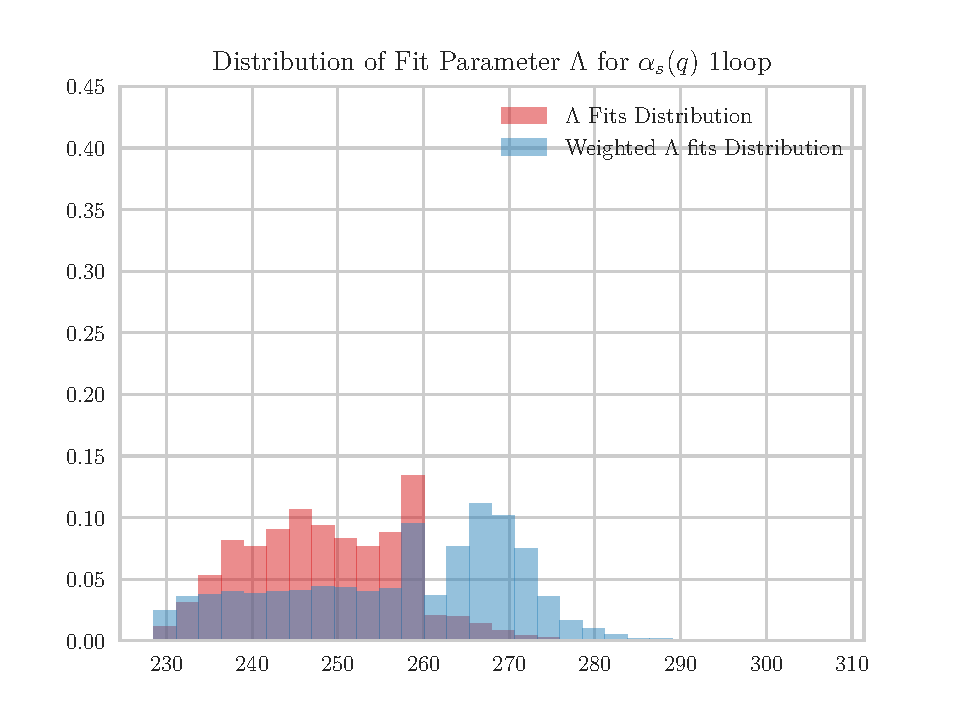
\includegraphics[width=1\textwidth]{results/hist1.pdf}
    \end{subfigure}
    \begin{subfigure}{0.49\textwidth}
        \centering
        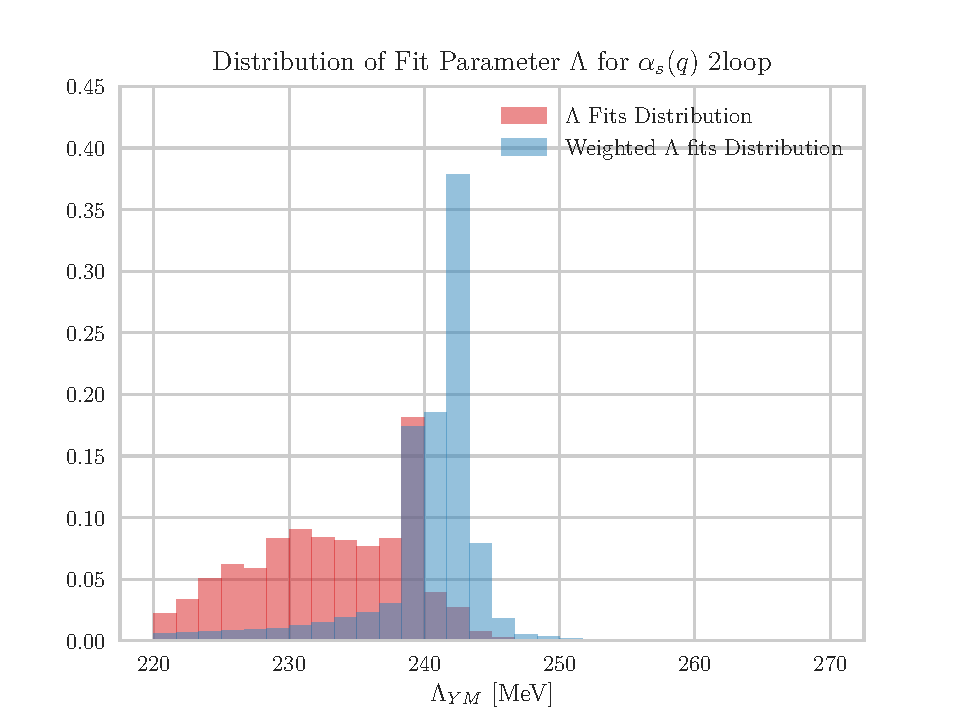
\includegraphics[width=1\textwidth]{results/hist2.pdf}
    \end{subfigure}

    \begin{subfigure}{0.49\textwidth}
        \centering
        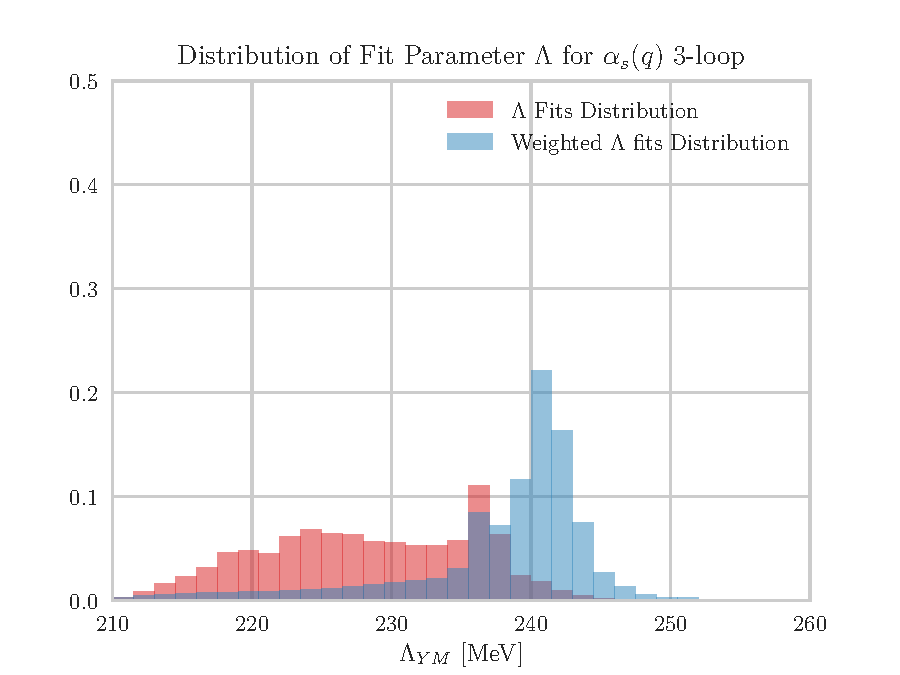
\includegraphics[width=1\textwidth]{results/hist3.pdf}
    \end{subfigure}
    \begin{subfigure}{0.49\textwidth}
        \centering
        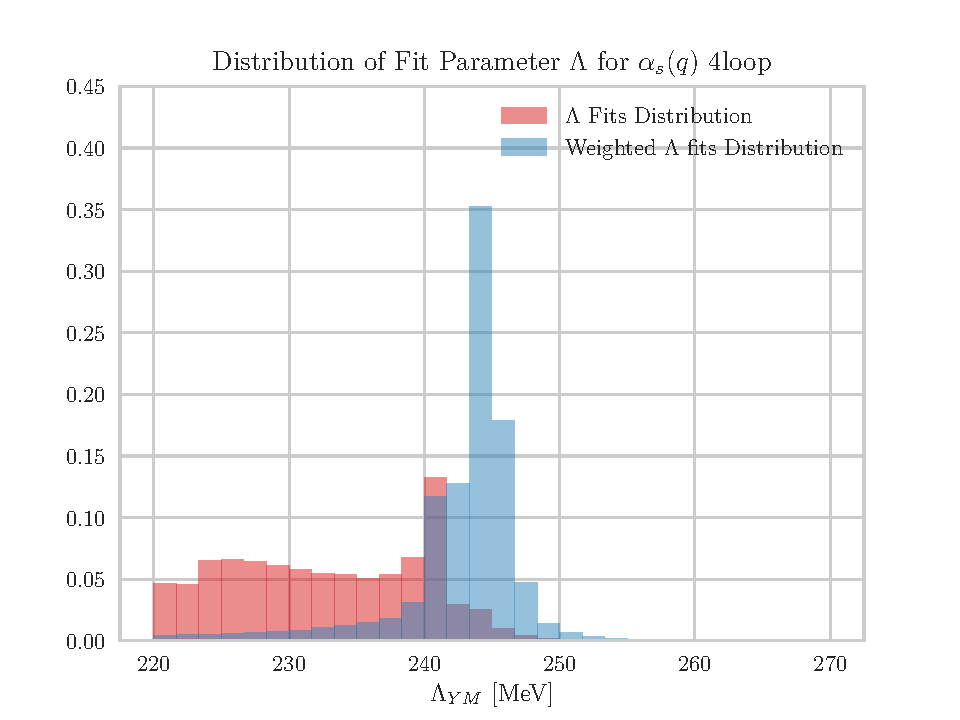
\includegraphics[width=1\textwidth]{results/hist4.pdf}        
    \end{subfigure}
    \caption{Distributions of the fit parameters, $\Lambda$, obtained by all possible fit ranges between $t_f/r_0^2 = 0.005$ to $0.085$ of minimum size $0.005$. The four different plots are for the four different orders of corrections for $\alpha_s(q)$. Data for the distribution weighted with $1/\chi^2$, normalized to the number of fits, is also reported.}
    \label{lambda_hist}
\end{figure}

The fact that the weighted distributions have a peak means that there is a certain region in the energy spectrum where the function in \cref{eq:t2Ebuona} matches the data better. This is expected since we know that for low energies perturbation theory does not hold anymore, so the function does not represent the data correctly. At high energies on the other hand, by looking at \cref{fig:t2EZoom} for example, the discretization effects introduced by the lattice method become relevant, so the continuum limit extrapolation that we made is unreliable in that region.\\
From the plot of the 1-loop corrected function, one can see that there is no sharp peak in the weighted distribution, compared to the others. The difference in the behavior is not surprising if one looks at \cref{fig:couplings} and considering that the higher order functions for $alpha_s(q)$ are all close together in the energy range considered. 

The estimation of the $\Lambda_{YM}$ scale is taken by considering the weighted median of the data, which is defined as the $50\%$ weighted percentile, the element $x_k$ of an ordered set of values $x_1, x_2, \dots, x_N$ that satisfies:
\beq
    \sum_{i=0}^{k-1} w_i \leq \frac{1}{2} ~~~~ \text{and}  ~~~~~ \sum_{i=k+1}^{N} w_i \geq \frac{1}{2}
\eeq
The systematic uncertainty has been taken as the $68\%$ confidence interval of the weighted median distribution, as it was done in \cite{durr_ab-initio_2008-1}. To estimate the statistical error, the whole procedure has been applied to 500 bootstrap samples of the lattice data, constructing the continuum limit limit for each sample and performing fits on all fit ranges for sample. The results are shown in \cref{table:lambda_table}.

\begin{table}[!htb]
    \begin{center}
        \capt{Final results for the scale $\Lambda_{YM}$ from the distribution of the fits in \cref{lambda_hist}. The results are shown as $r_0\Lambda_{YM}$, the dimensionless lattice value for the scale. The value of  $\Lambda_{YM}$ in MeV is taken by setting $r_0=0.5$ fm. The first value within brackets after one value is the systematic error, given by the width of the weighted fit distribution. The second value within brackets is the statistical error, estimated by the standard deviation of the weighted means of the bootstrap samples.}
        \begin{tabular}{ccc} 
            Fit Function Order & $r_0\Lambda_{YM}$ & $\Lambda_{YM}$ [MeV] \\\hline
            1-loop & $0.656(78)(17)$ & $259(31)(7)$ \\
            2-loop & $0.612(26)(2)$ & $242(10)(1)$  \\
            3-loop & $0.608(38)(3)$ & $239(15)(2)$  \\
            4-loop & $0.618(32)(2)$ & $244(13)(1)$  
        \end{tabular}
        \label{table:lambda_table} 
    \end{center} 
\end{table}

The statistical error is consistently smaller than the systematic. This means that the weighted fitting procedure is not affected by statistical fluctuations and that the outcome of the fit is reliable. However the rate of the errors also implies that almost all the uncertainty is given by the method used to estimate $\Lambda_{YM}$. \\
Perhaps unsurprisingly, the result for the one-loop corrected form of $\alpha_S(q)$ differs significantly from the higher order corrections. The uncertainty is also by far larger. However, this difference is easily explained by considering \cref{fig:couplings}, which shows that the distance between the one-loop expression for $\alpha_S(q)$ is significantly different from all the others. 
The values we found for $\Lambda_{YM}$ can now be compared with ones found in literature for the same quantity using different methods. In particular we compare it with the one found in \cite{capitani_non-perturbative_1999} obtained using a recursive finite-size technique, which is reported as $\Lambda_{ref} = 238(18)$ MeV. The values found in \cref{table:lambda_table} agree very well with the reference.\\ 
One last result to show is the plot of $t_f^2\langle E\rangle$ as function of $q$ using the perturbative expression, \cref{eq:t2Ebuona}, and our values of $\Lambda_{YM}$ as input. In \cref{fig:end,fig:end1} the function is plotted for every order, together with the continuum limit data extrapolated from the lattice. We can see that good agreement is found between $q \approx 700$ and $1600$ MeV, or in flow time between $t_f/r_0^2 \approx 0.008$ to $t_f/r_0^2 \approx 0.045$

\begin{figure}[hbt!]
    \centering
    \begin{subfigure}{0.7\textwidth}
        \centering
        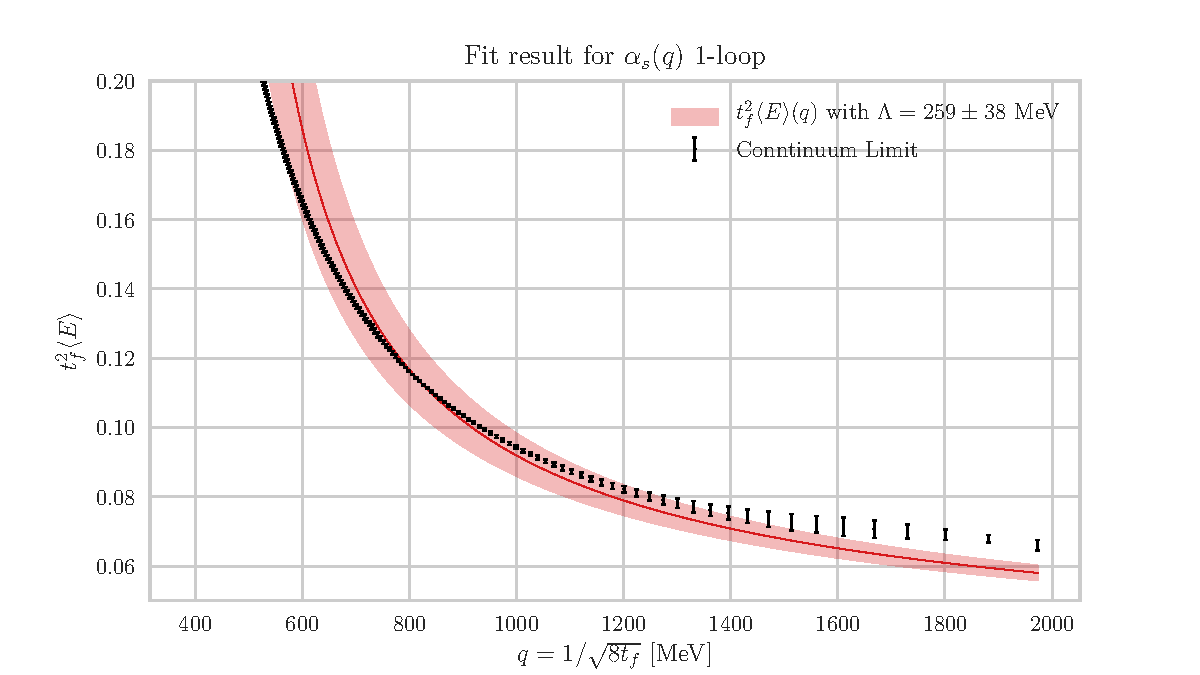
\includegraphics[width=1\textwidth]{results/End1.pdf}
    \end{subfigure}
    \begin{subfigure}{0.7\textwidth}
        \centering
        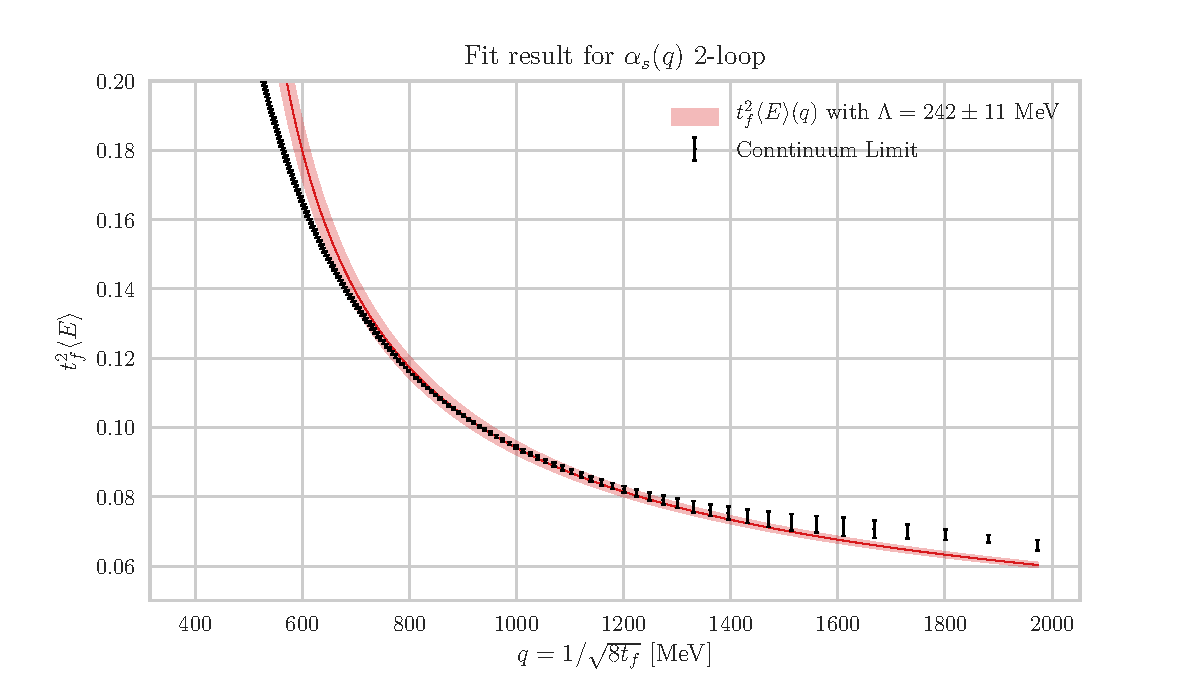
\includegraphics[width=1\textwidth]{results/End2.pdf}
    \end{subfigure}

    \caption{Plot of $t_f^2\langle E\rangle$, \cref{eq:t2Ebuona} as a function of the momentum scale $q$, using the values of the scale found in \cref{table:lambda_table}. The error band is the sum of the statistical and systematic errors from the same table. The data series in black is the continuum limit extrapolated from the lattice. On the top the function is plotted using the one-loop corrected expression for $\alpha_S(q)$ and $\Lambda_{YM} =259(31)(7)$ MeV. The bottom plot uses the two-loop corrected  $\alpha_S(q)$ and $\Lambda_{YM} =242(10)(1)$ MeV. Note that the plotted continuum function is the result of the multiple weighted fits procedure.}
    \label{fig:end}
\end{figure}
\begin{figure}[hbt!]
    \centering
    \begin{subfigure}{0.7\textwidth}
        \centering
        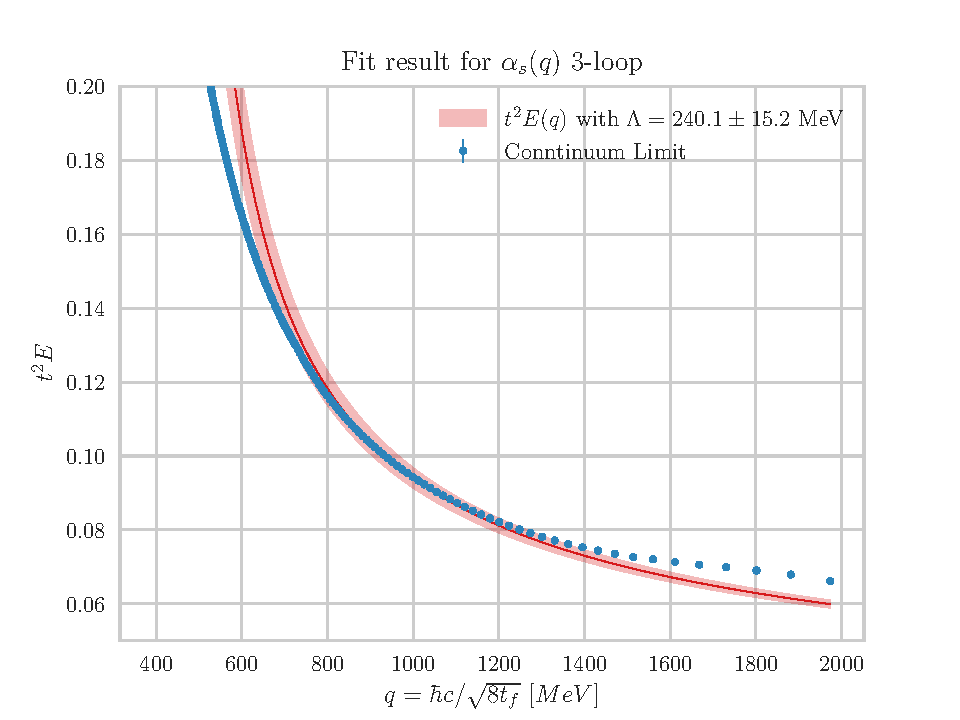
\includegraphics[width=1\textwidth]{results/End3.pdf}
    \end{subfigure}
    \begin{subfigure}{0.7\textwidth}
        \centering
        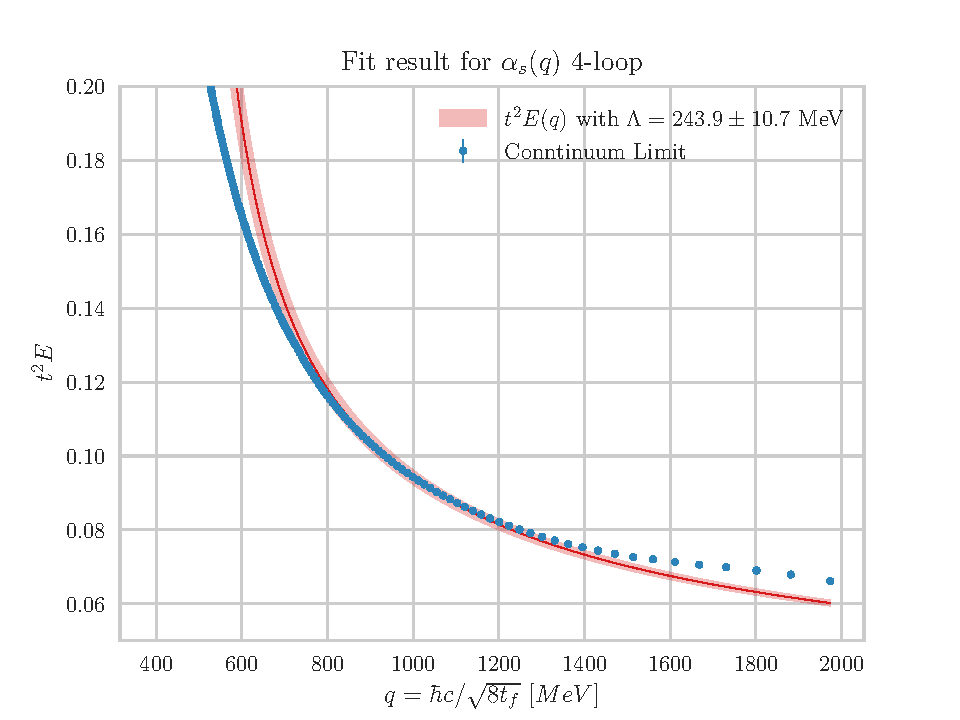
\includegraphics[width=1\textwidth]{results/End4.pdf}        
    \end{subfigure}
        \caption{Plot of $t_f^2\langle E\rangle$, \cref{eq:t2Ebuona} as a function of the momentum scale $q$, using the values of the scale found in \cref{table:lambda_table}. The error band is the sum of the statistical and systematic errors from the same table. The data series in black is the continuum limit extrapolated from the lattice. On the top the function is plotted using the three-loop corrected expression for $\alpha_S(q)$ and $\Lambda_{YM} =239(15)(2)$ MeV. The bottom plot uses the four-loop corrected  $\alpha_S(q)$ and $\Lambda_{YM} =244(13)(1)$ MeV. Note that the plotted continuum function is the result of the multiple weighted fits procedure.}
    \label{fig:end1}
\end{figure}

The conclusion we can make from these results is that there is clear agreement between the perturbative expansion in the coupling of $t_f^2\langle E\rangle$ and the continuum limit extrapolation that we performed for every flow time, in the intermediate energy range. At low values of $q$ as expected  the perturbative expansion diverges from the lattice data. As the coupling $\alpha_S(q)$ increases the less accurate perturbation theory becomes.\\
The more controversial data to interpret is the high-energy limit. In principle, once the continuum limit is recovered from the lattice data, the data should always be consistent with perturbation theory. However we see that our continuum limit extrapolation is systematically higher than the results of our fitting procedure.  \\
One possible check of this would be to only consider the high-energy points in the fit. The resulting fit however, would be very far from the data at smaller energies. By performing this check we found the value, in the case of four-loop-corrected $\alpha_S(q)$, $r_0\Lambda_{YM} = 709(31)$ MeV, which is a much worse estimate for the quantity, also basing the comparison on references \cite{capitani_non-perturbative_1999}. This is probably in indication that the high energy mismatch is most likely a flaw of the continuum limit extrapolation. A possible issue is for example highlighted in \cref{fig:extrapolation005}, where one can see that the final extrapolated value is affected by systematic errors introduced by the choice of which lattice spacings to fit. In a more general picture, this means that a proper estimation of the systematics of the extrapolation at low flow times is needed in order to recover the correct continuum limit at high energies.\\
One further remarks should be made on the procedure we used to find the best estimate of $\Lambda_{YM}$. The method of performing multiple fits over different windows of the momentum scale $q$ and the choice of weighting them with the fit quality, proved successful. In particular the assessment of the systematic uncertainty seems to be reasonable. A single fit over the whole energy range would have produced a very different result. However physically we expect the matching of the continuum limit data with the perturbative expansion of  $t_f^2\langle E\rangle$  to be better at high-energies, so a possible improvement could be to add some weights to the different fitting windows depending on their range, in order to give more importance to the fits performed at high $q$. 